\section{Quantum mechanics in a box}

The Schrödinger equation tells us the time-evolution of the wave function, which, according to the Copenhagen interpretation of quantum mechanics, has the physical interpretation of a probability amplitude when squaring the absolute value. In our current setup, where we have
\begin{equation} 
V = \begin{cases}
0,\quad 0<x<L \\
\infty,\quad \text{otherwise}
\end{cases},
\end{equation}
there is 0\% chance of finding the particle inside the ``walls'' (at $x<0$ or $x> L$). Thus, the wave function must go to zero at these points. Defining $x' = x/L$ and $t'=t/t_0$, and inserting in \cref{eq:SE}.
\begin{align*} 
i\hbar\pdv{\psi}{t} &= i\hbar\pdv{\psi}{t'}\pdv{t'}{t}= \frac{-\hbar^2}{2mL^2}\pdv[2]{\psi}{{x'}}\\
\implies i\pdv{\psi}{t'} &= \frac{-\hbar}{2mL^2 \pdv{t'}{t}}\pdv{\psi}{x'^2}
\end{align*}
Thus, setting
\begin{equation}
\label{eq:normalized_stuff}
t' = \frac{\hbar}{2mL^2}t,\quad x' = \frac{x}{L}
\end{equation}
gives the wanted dimensionless equation
\begin{equation}
\label{eq:SE_dimensionless}
i\pdv{\psi}{t'} = -\pdv[2]{\psi}{{x'}}.
\end{equation}
Inserting our new variables in \cref{eq:TISE} with \[H = \frac{\hat p^2}{2m} + V(x) =  -\frac{-\hbar}{2mL^2} \pdv[2]{{x'}} + \tilde{V}(x'),\] we get
\begin{align} 
\frac{-\hbar^2}{2mL^2}\pdv[2]{\psi_n}{{x'}} &= E_n\psi_n \implies \nonumber\\
\label{eq:eig}
-\pdv[2]{\psi_n}{{x'}} &= \lambda_n\psi_n,
\end{align}
with the relation 
\begin{equation} 
\label{eq:energy_conversion}
\lambda_n = \frac{2mL^2 E_n}{\hbar^2}
\end{equation}
between the energy levels and the dimensionless eigenvalues. The boundary conditions that the wave function disappears in the walls, but the walls are now at $x' = 0$ and $x' = 1$. It is now clear that choosing $x_0 = L$ is suitable, as it makes us able to work on the simple domain $[0,1]$. Any other proportionality constant $\alpha\in \mathbb{R}$ such that $x' = \alpha x/ L$ should work as well, scaling both the time and energies by a factor $\alpha^2 $, as long as $x'$ is dimensionless. Other scaling possibilities are also possible, and have consequences for the analytic expressions for $\psi$. For example scaling the interval to be mirrored about $x = 0$ would only pick out the even terms in a Fourier series expansion.

Solving \cref{eq:eig} with the imposed boundary conditions can be done analytically in the following manner.
Since we are looking for solutions that have self-similar second derivatives with an extra minussign, we guess a solution on the form 
$\psi = A_n\sin(\sqrt{\lambda_n}x') + B_n\cos(\sqrt{\lambda_n}x')$. The boundary condition $\psi(x'=0) = 0$ gives $B_n = 0$, while the boundary condition $\psi(x'=1) = 0$ gives the restriction to $\lambda_n$ that $\sqrt{\lambda_n} = n\pi$, hence the labels $n$ are also justified. Our analytic solution is therefore 
\begin{equation}
\label{eq:eigenfunc}
\psi_n(x') = \mathcal{N}\sin(\pi n x'),
\end{equation} 
where $\mathcal{N}$ is a normalization constant to be decided.
\begin{align*} 
1 &= \braket{\psi_n}{\psi_n} = \mathcal{N}^2\int_{0}^{1}\dd{x'}\sin[2](n\pi x') \\
&=\mathcal{N}^2\int_0^1\dd{x'}\frac{1-\cos(2\pi n x')}{2}
= \frac{\mathcal{N}^2}{2} \\
&\implies \mathcal{N} = \sqrt{2},
\end{align*}
and we have the analytic solution as announced in \cite{assignment}.

The implementation of a finite-difference-scheme is done using sparse matrix formatting for the cases when the discretization step is very small. Otherwise a dense matrix format is sufficient for solving eigenvalues, using the ``eigsh''-function from NumPy's linear algebra library.

\begin{figure}[tb]
	\centering
	\begin{subfigure}{0.5\textwidth}
	\centering
	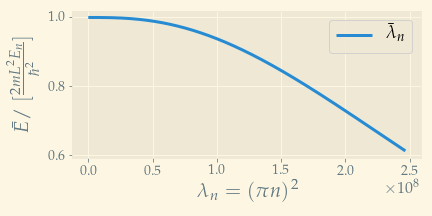
\includegraphics[width=\linewidth]{img/e_vs_lambda_N=5000}
	\caption{Computed eigenvalues against the analytic expression.}
	\end{subfigure}
	\hfill
	\begin{subfigure}{0.5\textwidth}
	\centering
	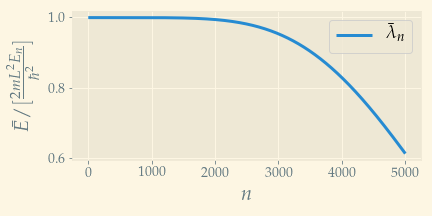
\includegraphics[width=\linewidth]{img/e_vs_n_N=5000}
	\caption{Computed eigenvalues against $n$.}
	\end{subfigure}
	\caption{Comparison of computed eigenvalues and the analytic expressions. }
	\label{fig:energy_comparison}
\end{figure}
In \cref{fig:energy_comparison} a comparison of the calculated eigenvalues against both the analytic expression for $\lambda_n$ and $n$ is shown for the case where the interval is discretized in 5000 points.  Notice that $\bar\lambda_n / \lambda_n$ is close to 1 for $n$ up to about 2000, where the energies are $2000^2$ times higher than the ground state.


To compute the error of a numerical solution, we must have a metric of some sort. Let us introduce
\begin{equation} 
E[\bar\psi_n(x')] = \int\dd{x'}||\bar \psi_n(x')|-|\psi_n(x')||^2
\end{equation}
as an example, where the bar denotes the numerical approximation to the analytic function.
Then, a comparison of the eigenvectors with respect to the number of discretization steps can be made. 
\begin{figure}
	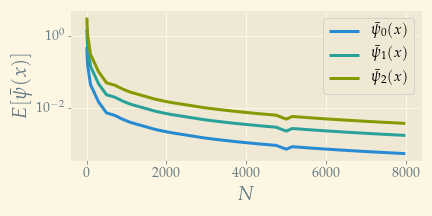
\includegraphics[width=\linewidth]{img/discretization_step.png}
	\label{fig:discretization}
	\caption{Error of the ground state, first- and second excited states as a function of the discretization steps.}
\end{figure}
In \cref{fig:discretization}, this is shown for the three lowest energy levels. 


The implementation of 
\begin{equation} 
\alpha_n = \braket{\psi_n}{\Psi_0} = \int\dd{x'}\psi_n^*(x')\Psi_0(x')
\end{equation}
can be done in a simple fashion by taking optimized inner-product implementations for general vectors, so calculating the actual integral is actually not needed. 
\begin{figure}
	\centering
	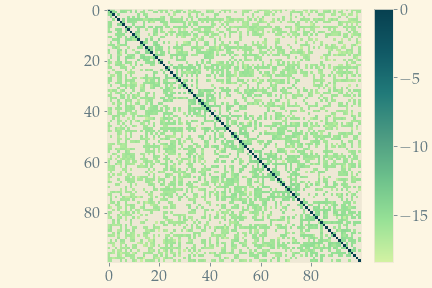
\includegraphics[width=\linewidth, trim={2.5cm 0 0 0}, clip]{img/ortho.png}
	\caption{Logarithm (base 10) of the inner product of the 100 lowest excited eigenfunctions.}
	\label{fig:orthogonality}
\end{figure}
In \cref{fig:orthogonality}, the inner product of the first 100 eigenfunctions are shown, and indicates orthogonality of the states. The off-diagonals are $\sim 15 $ orders of magnitude smaller than the diagonal, which we might attribute to numerical artifacts or the imperfectness of the solutions, which we have seen is present, c.f. \cref{fig:energy_comparison,fig:discretization}. 

Using the reduced units previously discussed, we can express the full state
\begin{equation} 
\Psi(x, t) = \sum_n\alpha_n\exp(-\frac{iE_n t}{\hbar})\psi_n(x)
\end{equation}
as
\begin{align} 
\sum_n\alpha_n\exp(-\frac{iE_n t}{\hbar})&\psi_n(x) =\sum_n\alpha_n\exp(-\frac{iE_n t}{\hbar})\psi_n(x)\nonumber \\[1.5ex]\nonumber =\sum_n&\exp(-\frac{i\frac{\hbar^2\lambda_n}{2mL^2}\frac{2mL^2t'}{\hbar}}{\hbar})\psi_n(x') \\[1.5ex]\implies \Psi(x', t')&= \sum_n\alpha_n\exp(-i\lambda_n t')\psi_n(x').\label{eq:full_state}
\end{align}
Now using the ground state
\begin{equation} 
	\label{eq:init}
\Psi_0 = \sqrt2\sin(\pi x)
\end{equation}
as initial condition, we can compute the full state. 
\begin{figure}
	\centering
	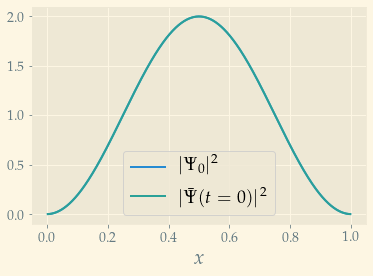
\includegraphics[width=\linewidth]{img/init_state}
	\caption{Analytic and computed probability density of initial state $\Psi_0$ using $N = 1000$ as the number of discretization points}
	\label{fig:init_state}
\end{figure}
In \cref{fig:init_state} the initial states are plotted both for the analytic expression and the computed value at $t = 0$.
The normalization is also well-defined, as seen in \cref{fig:normalization}.
\begin{figure}
	\centering
	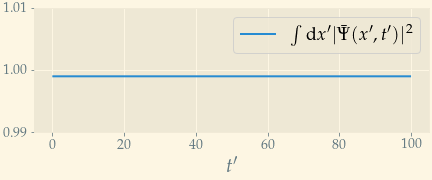
\includegraphics[width=\linewidth]{img/normalization.png}
	\caption{Normalization of the computed wave function for the time interval $t'\in [0,100]$ width $N =10000$ and $\Psi_0(x') = \delta(x'-\frac12)$.}
	\label{fig:normalization}
\end{figure}
For $\Psi_0$ as in \cref{eq:init}, this is expected, since $\Psi_0$ is orthogonal to $\Psi_{i\ne0}$, and $\Psi_0 $ is properly normalized itself. For $\Psi_0 = \delta(x'-1/2)$, however, this is more complicated. 
In this case, $c_n = \int\dd{x'}\psi_n^*\delta(x'-1/2)$
gives $c_n = \psi_n$, which means that only half of the eigenfunctions in \cref{eq:eigenfunc} will contribute. Numerically, however, we can only estimate the value of the Dirac-delta with a finite number of plane waves, in contrast to its integral representation $\delta \sim \int\dd{k}\e^{ikx}$.


